% Sandia National Laboratories is a multimission laboratory managed and
% operated by National Technology & Engineering Solutions of Sandia, LLC, a
% wholly owned subsidiary of Honeywell International Inc., for the U.S.
% Department of Energy’s National Nuclear Security Administration under
% contract DE-NA0003525.

% Copyright 2002-2020 National Technology & Engineering Solutions of Sandia,
% LLC (NTESS).


\begin{Device}

\symbol
{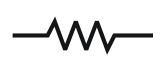
\includegraphics{resistorSymbol}}

\device
R<name> <(+) node> <(-) node> [model name] [value] [device parameters]

\model
\begin{alltt}
.MODEL <model name> R [model parameters]
.MODEL <model name> RES [model parameters]
\end{alltt}

\examples
\begin{alltt}
R1 1 2 2K TEMP=27
RM 4 5 R=4e3 M=2
RLOAD 3 6 RTCMOD 4.540 TEMP=85
.MODEL RTCMOD R (TC1=.01 TC2=-.001)
RSEMICOND 2 0 RMOD L=1000u W=1u
.MODEL RMOD R (RSH=1)
\end{alltt}

\parameters

\begin{Parameters}

\param{\vbox{\hbox{(+) node\hfil}\hbox{(-) node}}}

Polarity definition for a positive voltage across the resistor. The
first node is defined as positive. Therefore, the voltage across the
component is the first node voltage minus the second node voltage.
Positive current flows from the positive node (first node) to the
negative node (second node).

\param{model name}

If \texttt{[model name]} is omitted, then \texttt{[value]} is the
resistance in Ohms. If \texttt{[model name]} is given then the
resistance is determined from the model parameters; see the resistance
value formula below.

\param{value}

Positional specification of device parameter R (resistance).
Alternately, this can be specified as a parameter, \texttt{R=<value>},
or in the (optional) model.

\param{device parameters}

Parameters listed in Table~\ref{R_1_Device_Instance_Params} may be provided as
space separated \texttt{<parameter>=<value>} specifications as needed.
Any number of parameters may be specified.

\end{Parameters}

\comments

Resistors can have either positive or negative resistance values (R).  A zero 
resistance value (R) is also allowed. 

The power dissipated in the resistor is calculated 
with $I \cdot \Delta V$ where the voltage drop is calculated as $(V_+ - V_-)$ 
and positive current flows from $V_+$ to $V_-$.  The power accessors
(\texttt{P()} and \texttt{W()}) are supported for both the level 1 resistor
and the level 2 (thermal) resistor.

For compatibility with PSpice, either \texttt{R} or \texttt{RES} can be used in a
\texttt{.MODEL} statement for a resistor.

The Multiplicity Factor (\texttt{M}) can be used to specify multiple, identical 
resistors in parallel. The effective resistance becomes \texttt{R}/\texttt{M}.  
The \texttt{M} value need not be an integer.  It can be any positive real number.  
\texttt{M} can not be used as a model parameter. 

\end{Device}

\newpage
%\pagebreak

\paragraph{Device Parameters}
% This table was generated by Xyce:
%   Xyce -doc R 1
%
\index{resistor!device instance parameters}
\begin{DeviceParamTableGenerated}{Resistor Device Instance Parameters}{R_1_Device_Instance_Params}
DTEMP & Device Temperature -- For compatibility only. Parameter is NOT used & $^\circ$C & 0 \\ \hline
L & Length & m & 0 \\ \hline
M & Multiplicity Factor & -- & 1 \\ \hline
R & Resistance & $\mathsf{\Omega}$ & 1000 \\ \hline
TC1 & Linear Temperature Coefficient & $^\circ$C$^{-1}$ & 0 \\ \hline
TC2 & Quadratic Temperature Coefficient & $^\circ$C$^{-2}$ & 0 \\ \hline
TCE & Exponential Temperature Coefficient & \%$/^\circ$C & 0 \\ \hline
TEMP & Device temperature & $^\circ$C & Ambient Temperature \\ \hline
W & Width & m & 0 \\ \hline
\end{DeviceParamTableGenerated}


In addition to the parameters shown in the table, the resistor supports a vector parameter for the temperature correction coefficients.  \texttt{TC1=<linear coefficient>} and \texttt{TC2=<quadratic coefficient>} may therefore be specified compactly as \texttt{TC=<linear coefficient>,<quadratic coefficient>}.

\paragraph{Model Parameters}
% This table was generated by Xyce:
%   Xyce -doc R 1
%
\index{resistor!device model parameters}
\begin{DeviceParamTableGenerated}{Resistor Device Model Parameters}{R_1_Device_Model_Params}
DEFW & Default Instance Width & m & 1e-05 \\ \hline
NARROW & Narrowing due to side etching & m & 0 \\ \hline
R & Resistance Multiplier & -- & 1 \\ \hline
RSH & Sheet Resistance & $\mathsf{\Omega}$ & 0 \\ \hline
TC1 & Linear Temperature Coefficient & $^\circ$C$^{-1}$ & 0 \\ \hline
TC2 & Quadratic Temperature Coefficient & $^\circ$C$^{-2}$ & 0 \\ \hline
TCE & Exponential Temperature Coefficient & \%$/^\circ$C & 0 \\ \hline
TNOM & Parameter Measurement Temperature & $^\circ$C & Ambient Temperature \\ \hline
\end{DeviceParamTableGenerated}


Note: There is no model parameter for Default Instance Length.  The use of the semiconductor resistor model requires
the user to specify a non-zero value for the instance parameter \texttt{L}. 

\paragraph{Resistor Equations}

\subparagraph{Resistance Value Formulas}
If the \textrmb{R} parameter is given on the device instance line 
then that value is used.

If the \textrmb{R} parameter is not given then the semiconductor resistor model
will be used if the \textrmb{L} instance parameter and the \textrmb{RSH} model parameter
are given and both are non-zero.  In that case the resistance will be as follows.
(Note: If \textrmb{W} is not given on the instance line then the value
for the model parameter \textrmb{DEFW} will be used instead.)

\[
\mathbf{RSH} \frac{[\mathbf{L} - \mathbf{NARROW}]}
{[\mathbf{W} - \mathbf{NARROW}]}
\]

If neither of these two cases apply then the default value for
the \textrmb{R} parameter will be used.     

\subparagraph{Temperature Dependence}
If \textrmb{TCE} is specified as either an instance or model parameter
for the Level 1 resistor then the resistance at temperature $T$
is given by (where the resistance at the nominal temperature ($T_{0}$) 
was defined above in the resistance value formulas):

\[
\mathbf{R} \cdot pow(1.01,\mathbf{TCE} \cdot (T - T_{0}))
\]

otherwise the resistance is given by:
\[
\mathbf{R} \cdot (1 + \mathbf{TC1} \cdot (T - T_{0}) + \mathbf{TC2}
\cdot (T - T_0)^2)
\]

\paragraph{Thermal (level=2) Resistor}

\Xyce{} supports a thermal resistor model, which is associated with level=2.

\paragraph{Thermal Resistor Instance Parameters}
% This table was generated by Xyce:
%   Xyce -doc R 2
%
\index{resistor!device instance parameters}
\begin{DeviceParamTableGenerated}{Resistor Device Instance Parameters}{R_2_Device_Instance_Params}
A & Area of conductor & m$^{2}$ & 0 \\ \hline
DENSITY & Resistor material density (unused) & kg/$\mbox{m}^3$ & 0 \\ \hline
HEATCAPACITY & Resistor material volumetric heat capacity & $J/(\mbox{m}^3{}$K) & 0 \\ \hline
L & Length of conductor & m & 0 \\ \hline
M & Multiplicity Factor & -- & 1 \\ \hline
OUTPUTINTVARS & Debug Output switch & -- & false \\ \hline
R & Resistance & $\mathsf{\Omega}$ & 1000 \\ \hline
RESISTIVITY & Resistor material resistivity & $\mathsf{\Omega}$ m & 0 \\ \hline
TEMP & Device temperature & $^\circ$C & Ambient Temperature \\ \hline
THERMAL\_\-A & Area of material thermally coupled to conductor & m$^{2}$ & 0 \\ \hline
THERMAL\_\-HEATCAPACITY & Volumetric heat capacity of material thermally coupled to conductor & $J/(\mbox{m}^3{}$K) & 0 \\ \hline
THERMAL\_\-L & Length of material thermally coupled to conductor & m & 0 \\ \hline
W & Width of conductor & m & 0 \\ \hline
\end{DeviceParamTableGenerated}



%%
%% Resistor Model Param Table
%%
\paragraph{Thermal Resistor Model Parameters}
% This table was generated by Xyce:
%   Xyce -doc R 2
%
\index{resistor!device model parameters}
\begin{DeviceParamTableGenerated}{Resistor Device Model Parameters}{R_2_Device_Model_Params}
DEFW & Default Instance Width & m & 1e-05 \\ \hline
DENSITY & Resistor material density (unused) & kg/$\mbox{m}^3$ & 0 \\ \hline
HEATCAPACITY & Resistor material volumetric heat capacity & $J/(\mbox{m}^3{}$K) & 0 \\ \hline
NARROW & Narrowing due to side etching & m & 0 \\ \hline
R & Resistance Multiplier & -- & 1 \\ \hline
RESISTIVITY & Resistor material resistivity & $\mathsf{\Omega}$ m & 0 \\ \hline
RSH & Sheet Resistance & $\mathsf{\Omega}$ & 0 \\ \hline
TC1 & Linear Temperature Coefficient & $^\circ$C$^{-1}$ & 0 \\ \hline
TC2 & Quadratic Temperature Coefficient & $^\circ$C$^{-2}$ & 0 \\ \hline
TCE & Exponential Temperature Coefficient & \%$/^\circ$C & 0 \\ \hline
THERMAL\_HEATCAPACITY & Volumetric heat capacity of material thermally coupled to conductor & $J/(\mbox{m}^3{}$K) & 0 \\ \hline
TNOM & Nominal device temperature & $^\circ$C & Ambient Temperature \\ \hline
\end{DeviceParamTableGenerated}


The temperature model for the thermal resistor will be enabled
if the \textrmb{A} and \textrmb{L} instance parameters are 
given and the parameters \textrmb{HEATCAPACITY} and
\textrmb{RESISTIVITY} are also given as a pair of either 
instance parameters or model parameters.  Otherwise, the
resistance value and temperature dependence of the Level 2
resistor will follow the equations for the Level 1 resistor 
given above, with the caveat that \texttt{TCE} is only 
allowed as a model parameter for the Level 2 resistor.

If the temperature model for the Level 2 resistor is enabled,
then the resistance ($R$) is given by the following, where the 
\textrmb{RESISTIVITY} can be a temperature-dependent expression:

\[
\frac{\mathbf{RESISTIVITY} \cdot \mathbf{L}}
{\mathbf{A}}
\]

The rate-of-change ($dT/dt$) of the temperature ($T$) of the 
thermal resistor with time is then given by the following where 
$i_{0}$ is the current through the resistor:

\[
\frac{i_{0} \cdot i_{0} \cdot R}
{(\mathbf{A} \cdot \mathbf{L} \cdot \mathbf{HEATCAPACITY}) +
 (\mathbf{THERMAL\_A} \cdot \mathbf{THERMAL\_L} \cdot \mathbf{THERMAL\_HEATCAPACITY})}
\]
